% !TeX root = ../solution.tex

\hypertarget{he22.33}{%
\chapter{[HE22.33] City Trip 2}\label{he22.33}}

\begin{marginfigure}
	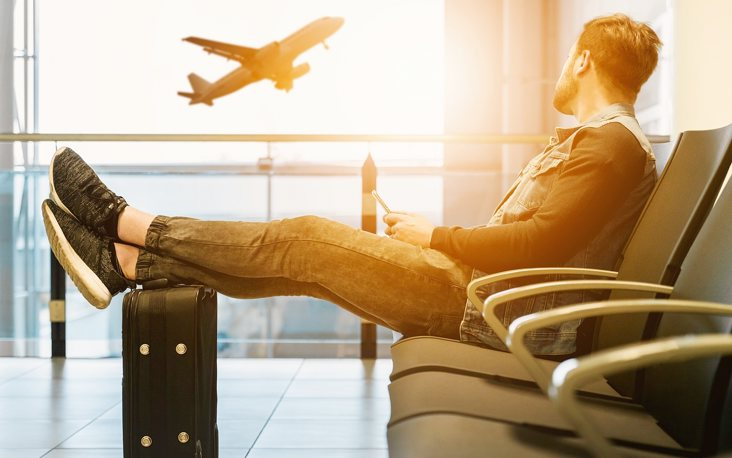
\includegraphics[width=49mm]{level7/challenge33.jpg}
\end{marginfigure}
\section{Intro}
Later that year, I was travelling again. Find out where I shot this picture!
This time, I want GPS coordinates.

\noindent {\NotoEmoji 🚩} Flag
\begin{itemize}
\item GPS coordinates, rounded to three decimals
\item  , as separator
\item  . as decimal point
\item  example:
\begin{itemize}
\item  40°46'30.3"N 73°57'59.8"W
\item  40.775082, -73.966599
\item  \verb+he2022{40.775,-73.967}+
\end{itemize}	
\end{itemize}	

\begin{marginfigure}
	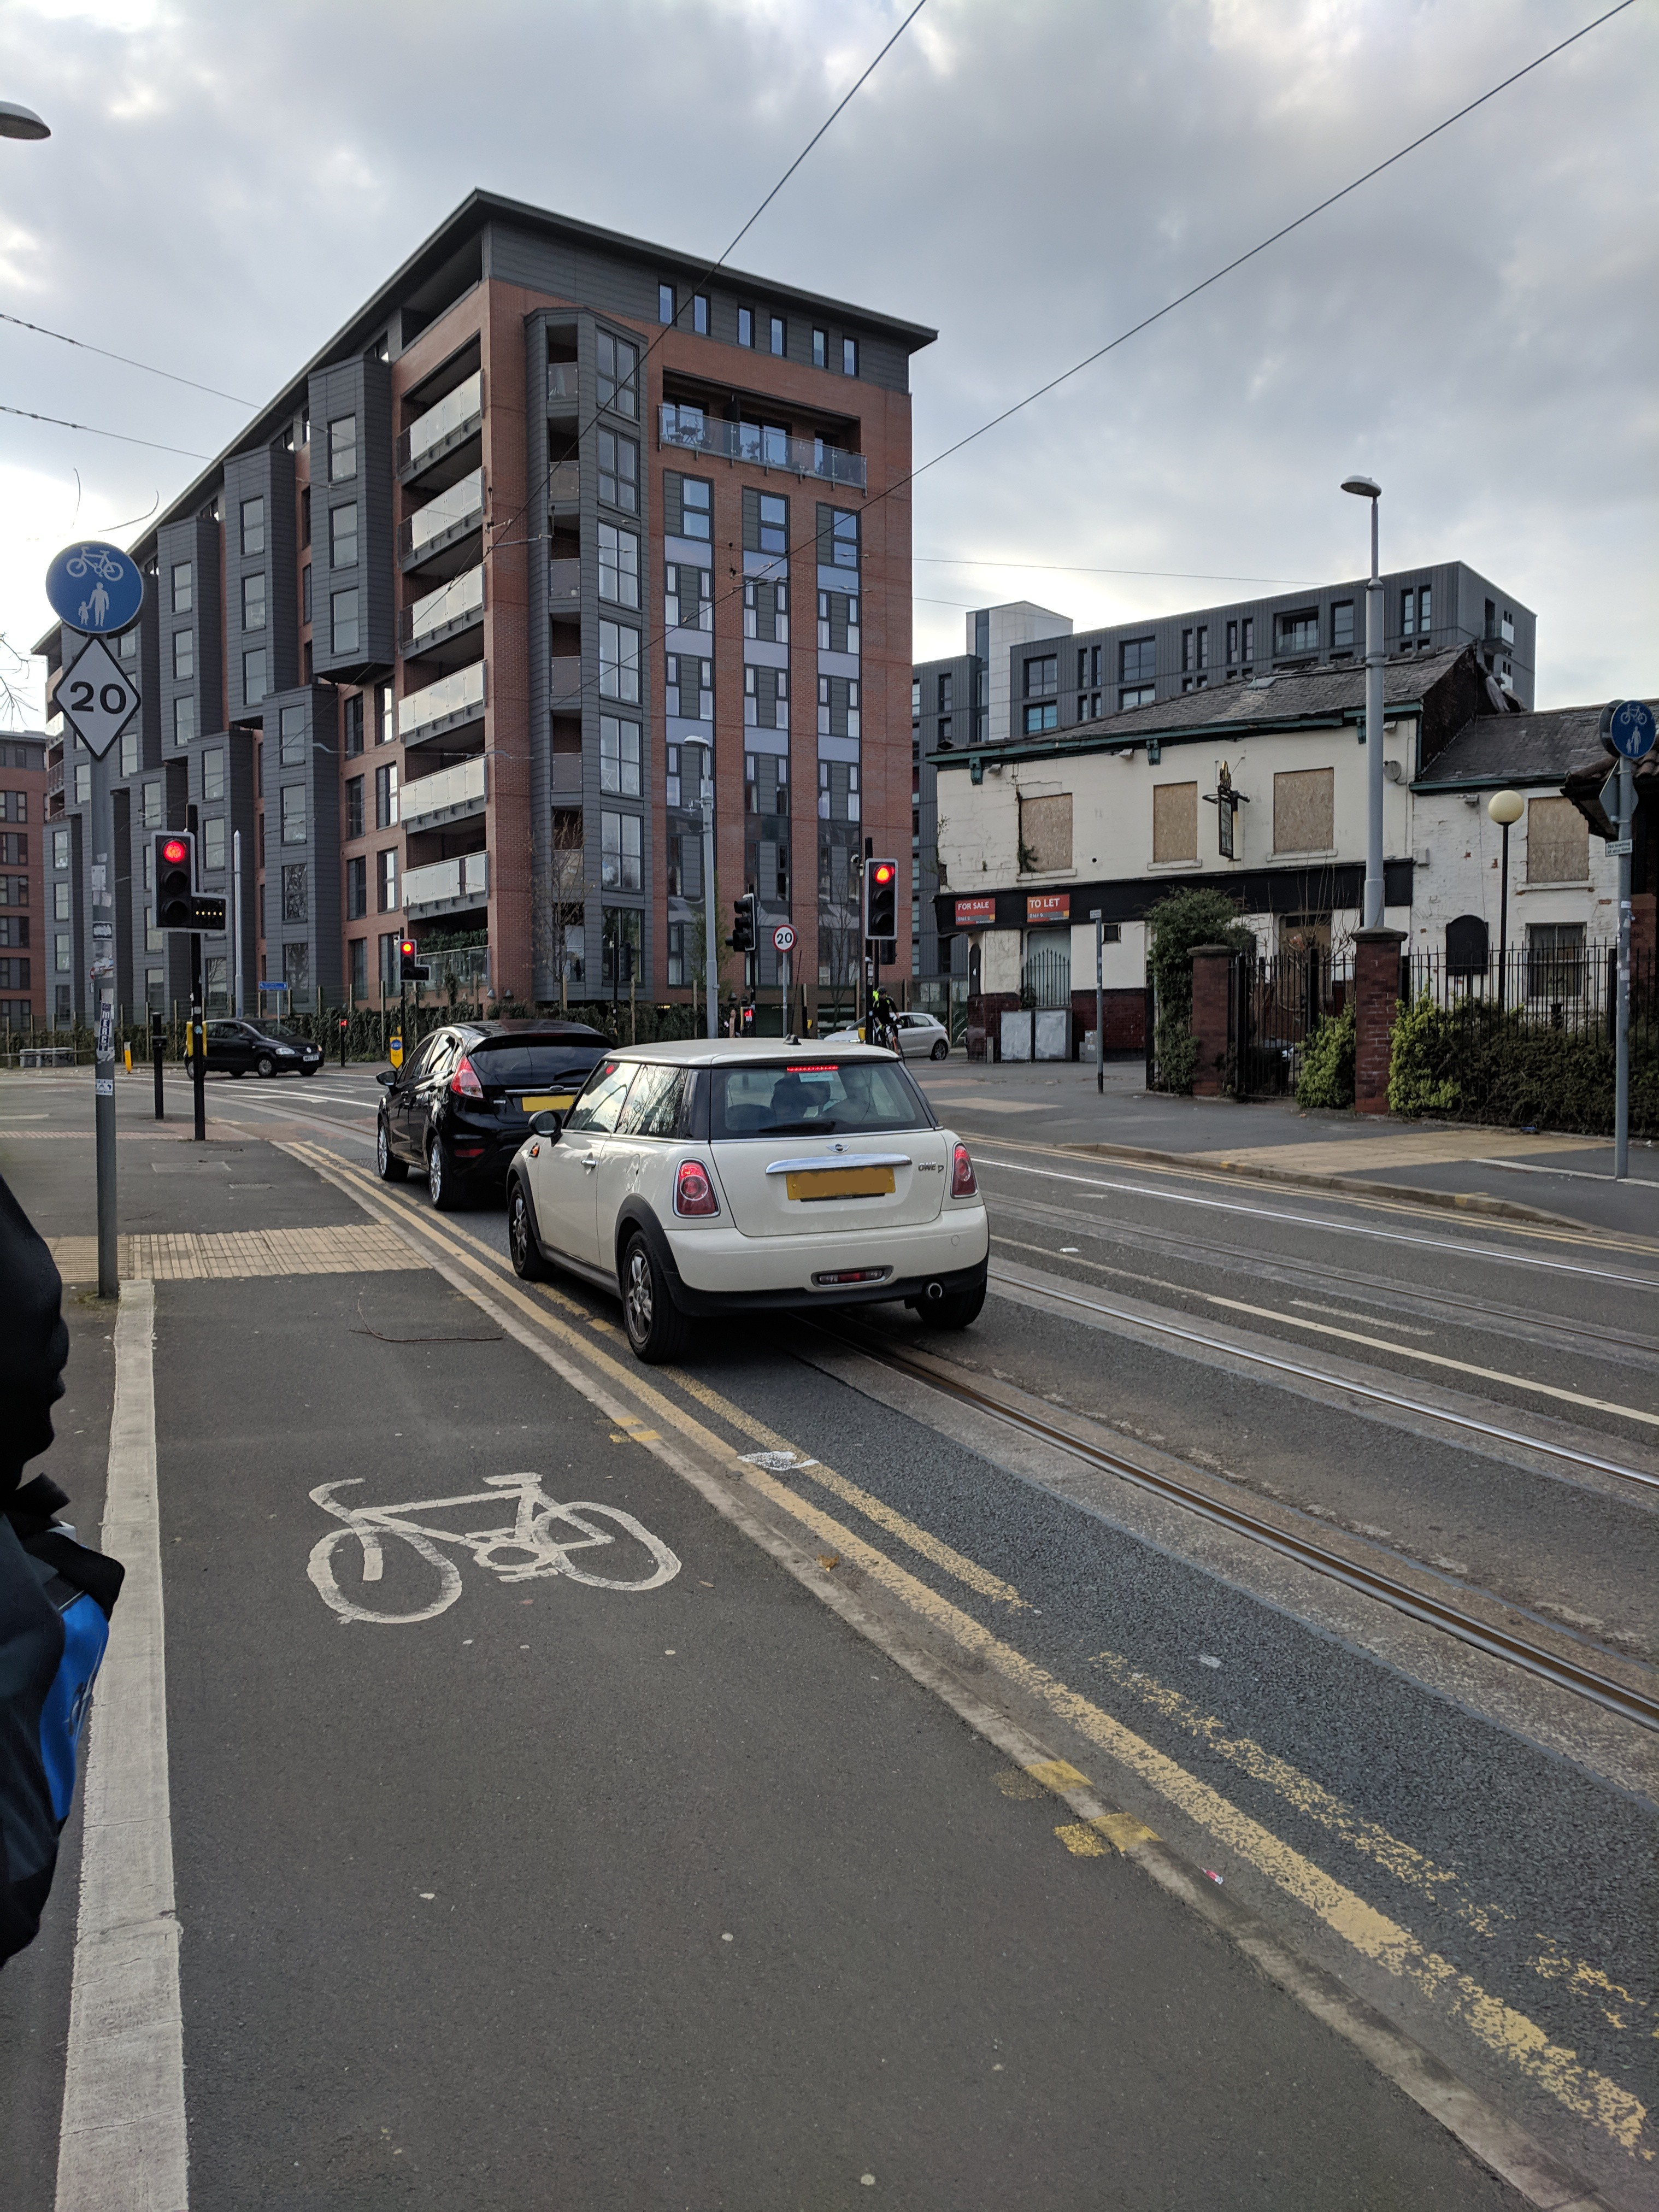
\includegraphics[width=49mm]{level7/citytrip2.jpg}
\end{marginfigure}



\section{Solution}\label{hv22.33solution}

\begin{marginfigure}
	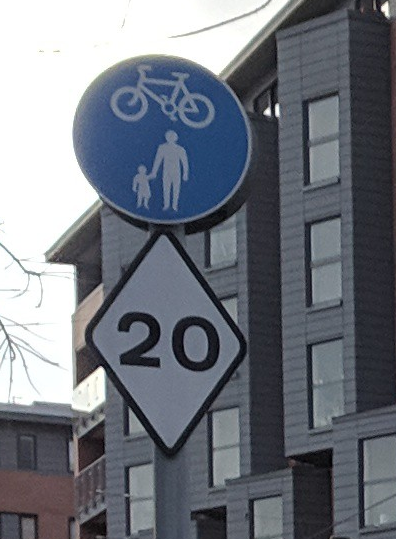
\includegraphics[width=49mm]{level7/street_sign.png}
\end{marginfigure}


We are given a photograph of a street corner.  Some things come out at once:
\begin{itemize}
\item the photo is taken in an English-speaking area
\item the license plates on the cars look European and not North American
\item the cars seem to drive on the left side of the road
\item there are tram-lines and a street sign indicating a speed limit for trams
	of 20mph
\item there are two signs on a dilapedated building ``for sale'' and ``to let''
	with telephone numbers showing an area code for Greater Manchester
\end{itemize}
All of these clues indicate that the street corner sought is somewhere in
Manchester, UK.  Check google maps in 2D mode where the tramlines are indicated
on the map and do a visual search for a place that looks like what we expect to
find from the photograph (tramlines on the street and on a slight corner), take
a look at the street view to verify, and we find the co-ordinates to get the
flag: \verb+he2022{53.482,-2.216}+





	









